Based on the findings in Chapter \ref{chp3}, it was determined that Machine Learning (ML) would be a suitable method for classifying the data obtained from the Pozyx system. Prior to attempting any experimentation, this chapter will conduct a survey of the current ML techniques available for the classification of Time Series Data. 


\section{Classic Machine Learning Methods}
\subsection{k-Nearest Neighbours (kNN)}
\subsubsection{Overview}
The k-Nearest Neighbours is a classifier that assigns a class to an unlabeled observation by looking at the class of $k$ neighbours and choosing the class that appears the most within these $k$ neighbours. The "nearest neighbours" are determined through a measure of Euclidean-Distance $D$ between a neighbour $p$ and unlabeled point $q$ with $n$ features is shown in Equation \ref{eq:distance} \cite{zhangIntroductionMachineLearning2016}

\begin{equation}
    D(p, q) = \sqrt[]{(p_1 - q_1)^2 + (p_1 - q_2)^2 + ... (p_n - q_n)^2}
    \label{eq:distance}
\end{equation}

Using Equation \ref{eq:distance} the top $k$ neighbours with the lowest distance are considered and the class that occurs the most within these nearest neighbours is the class chosen for the unlabeled observation. In the event that there is a tie between the classes, resolution of the tie depends on the implementation of the library used. In R kNN() resolves ties by picking a random tied candidate class \cite{zhangIntroductionMachineLearning2016} and scikit-learn's kNeighboursClassifier uses scipy's "mode" method which returns the first class that ties in the array \cite{ScipyStatsMode}.

\subsubsection{Dynamic Time Warping (DTW) as a Distance}
Though Euclidean-Distance may be suitable for problems with a fixed feature set, or vectors with the same length, patterns that manifest in time-series data may be stretched, compressed, or shifted in the temporal domain. Using Euclidean distance, a signal compared with the same signal shifted $t+1$ may result in large distances even though the signals compared were the same signals \cite{faouziTimeSeriesClassification2024}. A method called Dynamic Time Warping (DTW), was devised to counter the shortcomings of Euclidean distance and is robust to temporal variation that occurs naturally. It achieves this by calculating all the distances from one point to every other point and chooses a path that costs the least, finding the minimum distance between two vectors that do not ha e to be the same length. Mathematically, for $X = (x_1, x_2, ..., x_n)$ and $Y = (y_1, y_2, ..., y_m)$ be two time series of length $n$ and $m$ respectively, DTW first begins with calculating the Cost Matrix which is the cost between each pair in the time series \cite{faouziTimeSeriesClassification2024}  

\begin{equation}
    \forall_i \in {1,...,n}, \forall_j \in {1,...,n}, C_{ij} = f(i, j) 
\end{equation}

Where $f$ is the squared Euclidean-Distance (equation \ref{eq:distance} squared) for multivariate time-series \cite{faouziTimeSeriesClassification2024}.

\begin{equation}
    f(x, y) = D(x, y)^2
\end{equation}

A warping path is defined as $p = (p_1, ..., p_L)$ through the cost matrix $C$ begins on $p_1 = (1,1)$, must end on $p_L = (n, m)$ and moves with step $p_{l+1} - p_1 \in \{(1,0), (1,1), (0,1)\}$. The costs in the along the paths are summed And the DTW score is the path that costs the least \cite{faouziTimeSeriesClassification2024}.

\begin{equation}
    DTW(X, Y) = \min_{p \in P} C_p(X, Y) 
\end{equation}

Though every path does not need to be calculated as dynamic programming can be leveraged, the time complexity is still high at $O(nm)$ \cite{faouziTimeSeriesClassification2024} and this time complexity must be considered when designing a real-time classification system.

\subsubsection{Tunable Parameters}
The tunable parameter in kNN is $k$ and controls the number of neighbours selected. The optimal $k$ should be empirically chosen by varying $k$ for the selected dataset. When using kNN, the entire training dataset is used as-is. Therefore, class imbalance should also be considered. For example, a higher number of class A than class B could lead to a higher density of class A. Even though the unlabeled observation may be closer to class B, the classifier may choose class A because class B has "run out" of neighbours. With increasing $k$, the inaccuracy caused by class imbalance becomes even more apparent. If $k$ exceeds the number of samples in the class with the lower number of samples, then the class with the higher number of samples will always be chosen.

\subsection{Support Vector Machines (SVM)}
\subsubsection{Overview}
Support Vector Machines (SVM) involves finding a hyperplane that best separates 2 classes. There are two cases, the linearly separable case and the non-linearly separable case. In the linearly separable case, the hyperplane perfectly separates the two classes (see Figure \ref{fig:svm-hyperplane}). The idea is to maximize the "margin" which is the training data that is closest to the hyperplane \cite{cervantesComprehensiveSurveySupport2020}. Cervantes et al. depict this as maximizing the distance between parallel hyperplanes H1 and H2 (which pass through the "support vector" data-points of the training dataset) in Figure \ref{fig:svm-hyperplane} to optimize the generalization capability of the model.

\begin{figure}[ht]
    \centering
    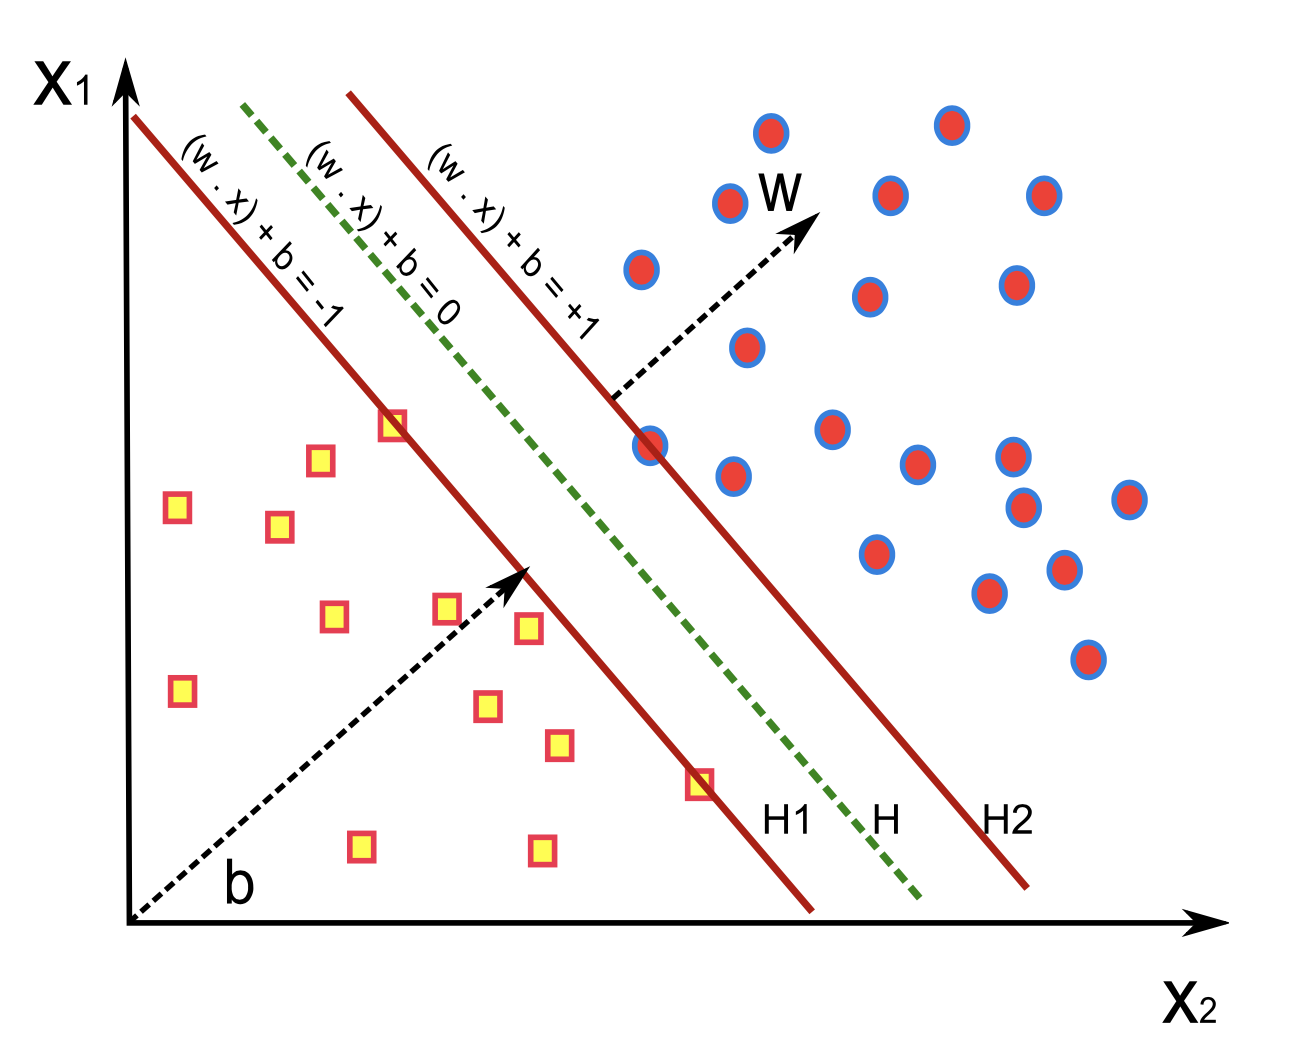
\includegraphics[width=0.6\textwidth]{SVM linearly separable.png}
    \caption{SVM Best Hyperplane in the linearly separable case \cite{cervantesComprehensiveSurveySupport2020}.}
    \label{fig:svm-hyperplane}
\end{figure}

The linearly separable case is rare in real life. Instead, datapoints from one class may seem to mix with the other class at the optimal boundary (Figure \ref{fig:svm-hyperplane-non-linearly-separable}). To still find this optimal boundary, a positive slack factor $\zeta_i$ is introduced and controlled by a parameter $C$ that controls the width of the margin. A lower $C$ allows for a wider margin that may improve generalizability in real life at the cost of more misclassification of the training datatset, whereas a higher $C$ tightens the margin and minimizes the classification errors in the training dataset but may decrease generalizability in real life \cite{cervantesComprehensiveSurveySupport2020}.  

\begin{figure}[ht]
    \centering
    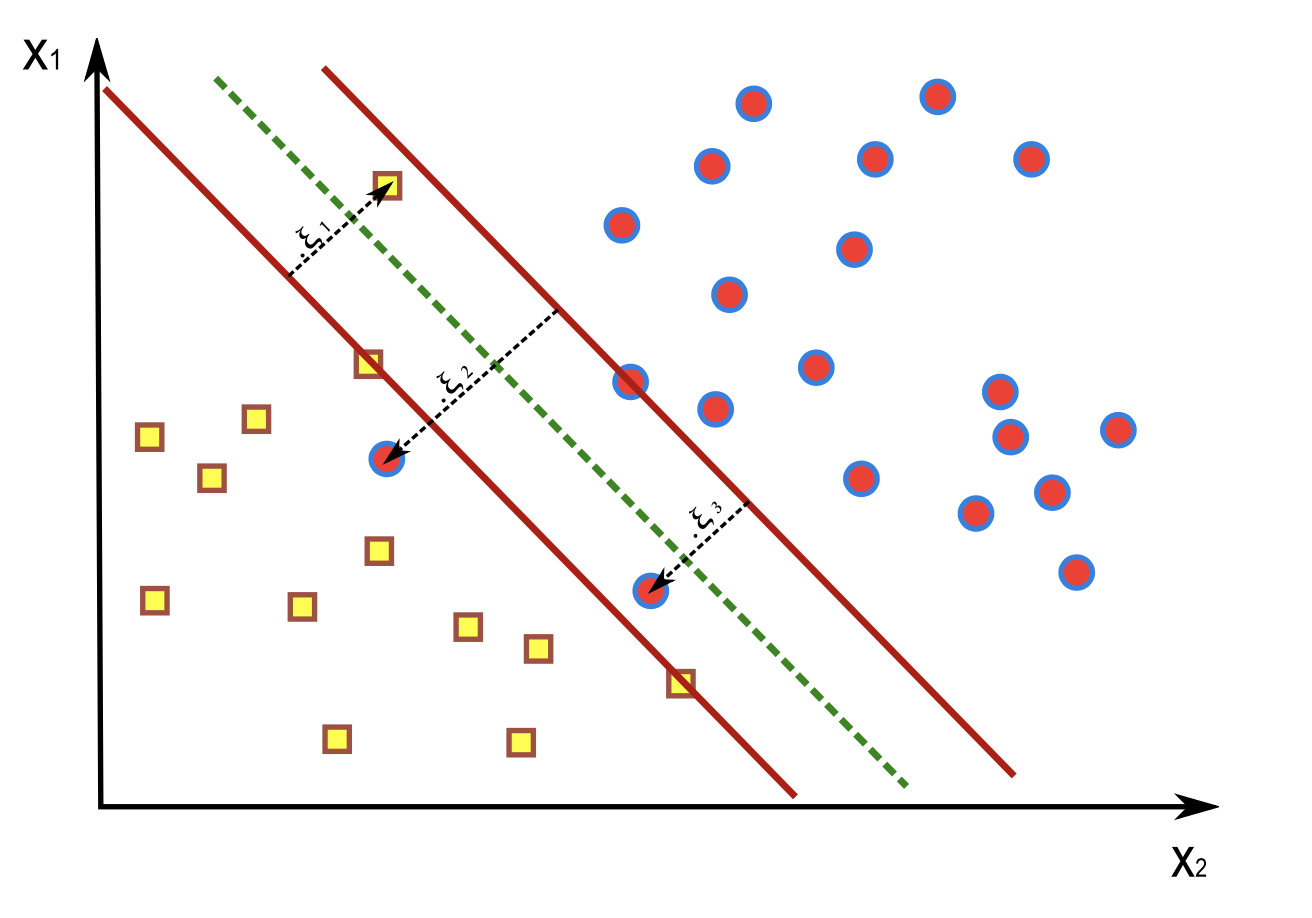
\includegraphics[width=0.6\textwidth]{SVM non-linearly separable.png}
    \caption{SVM Best Hyperplane in the non linearly separable case \cite{cervantesComprehensiveSurveySupport2020}.}
    \label{fig:svm-hyperplane-non-linearly-separable}
\end{figure}

SVM can also be used separate data that is not separable by a linear hyperplane (Figure \ref{fig:svm-hyperplane-non-linearly-classifier}) by using a kernel. Kernels reframe the problem in a highly dimensional space called the "feature space" and in this feature space, it is simple for the algorithm to find the hyperplane. In the next subsection that will detail the convex optimization problem for SVM, it is found that the function that needs to be optimized depends on the inner product between every sample $\langle x_i \cdot x_j \rangle$. Transforming the original dataset to this feature space through a transfer function $\phi$ yields an optimization problem that depends on $\langle \phi(x_i) \cdot \phi(x_j) \rangle$. Kernel functions $K(x_i, x_j)$ are special functions that provide an equivalent way to calculate $\phi(x_i) \cdot \phi(x_j)$ (ie $\phi(x_i) \cdot \phi(x_j) = K(x_i, x_j)$) without having to initially transform the original dataset using $\phi$ since transforming the dataset to the feature space may be a costly operation if there are many features. The following are popular kernels \cite{cervantesComprehensiveSurveySupport2020}:

\begin{enumerate}
    \item Linear Kernel: $K(x_i, x_j) = x_i \cdot x_j$
    \item Polynomial Kernel: $K(x_i, x_j) = (1 + x_i \cdot x_j)^p$
    \item Gaussian Kernel: $K(x_i, x_j) = e^{-\frac{{\left\lVert x_i - x_j\right\rVert}^2}{2\sigma^2}}$
    \item RBF Kernel: $K(x_i, x_j) = e^{-\gamma(x_i - x_j)^2}$
    \item Sigmoid Kernel: $K(x_i, x_j) = tanh(\eta x_i \cdot x_j + v )$
\end{enumerate}

\begin{figure}[ht]
    \centering
    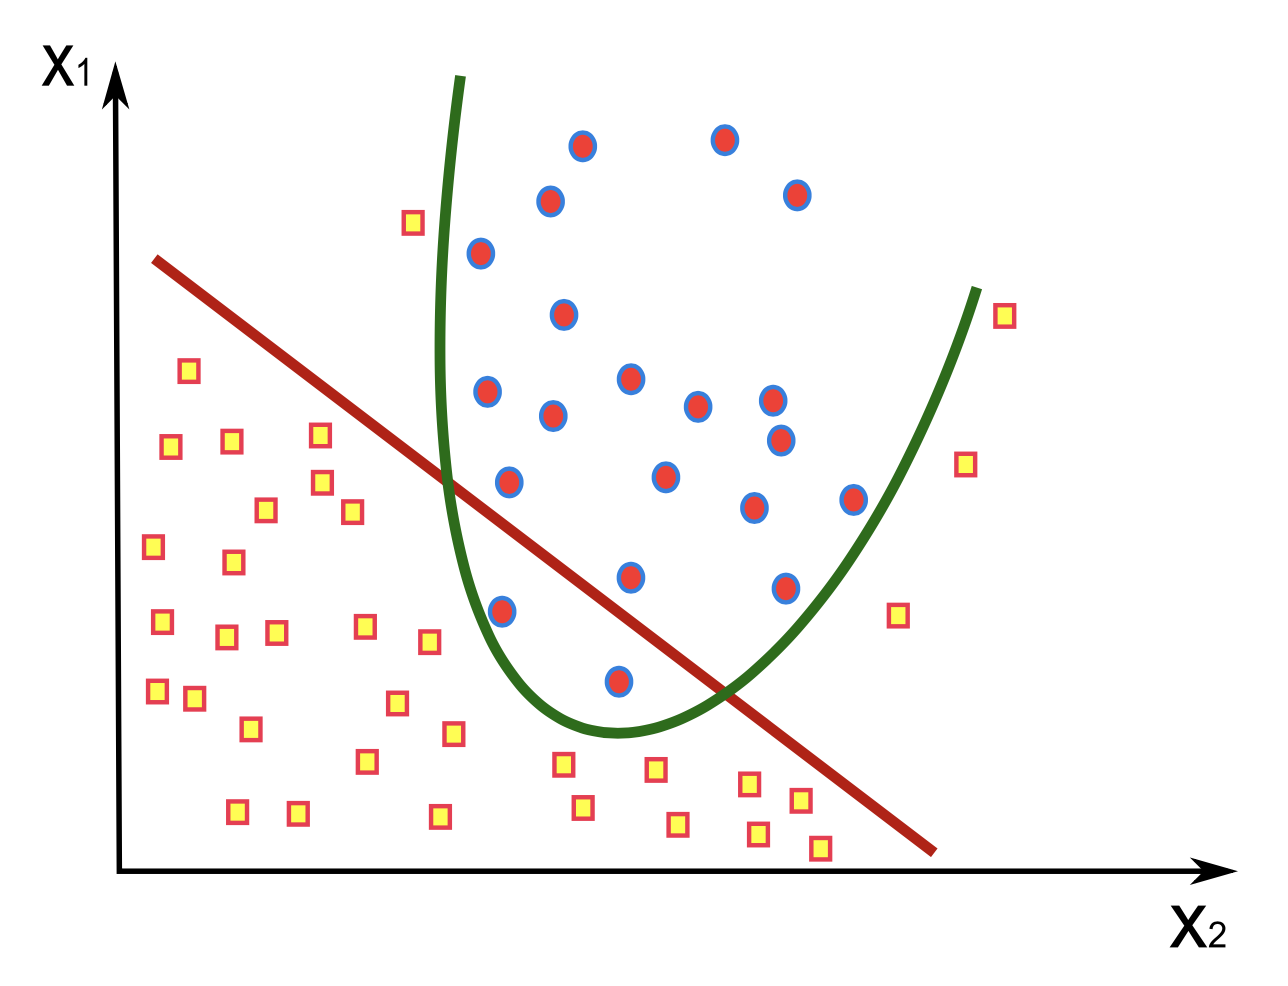
\includegraphics[width=0.6\textwidth]{SVM non-linear classifier.png}
    \caption{SVM non-linear classifier (green line) \cite{cervantesComprehensiveSurveySupport2020}.}
    \label{fig:svm-hyperplane-non-linearly-classifier}
\end{figure}

Since SVM can only separate between 2 classes as a binary classifier, a further step must be done to separate multiple classes. Scikit-learn uses a one vs. rest strategy by default. For each class a decision boundary between itself and the rest of the samples are created. For an unlabeled point a probability of membership to each class is calculated and an argmax function is used to determine the membership \cite{12MulticlassMultioutput}.

\clearpage
\subsubsection{Theory of SVM: Linearly Separable}
Consider a training dataset $X = \{x_i, y_i\}^n_{i=1}$ consisting of $n$ samples of feature vectors $x_i \in \mathbb{R}$ and labels $y_i \in (-1, 1)$. In the linearly separable case of SVM, the two classes in our training dataset can be separated perfectly by a hyperplane. The data labelled with class $y=1$ will be on one side of the hyperplane and the other class $y=-1$ will be on the other side of the hyperplane. The equation for a hyperplane is given in Equation \ref{eq:hyperplane}

\begin{equation}
    \mathbf{w \cdot x} + b = 0
    \label{eq:hyperplane}
\end{equation}

Where $x \in \mathbb{R}^d$, and $\mathbf{w}$ the weights for the hyperplane and $b$ the bias. For simplicity of visualization, consider $x \in \mathbb{R}^2$. The SVM optimization problem tries to find $\mathbf{w}$ and $b$ such that the margin (ie. the distance to the closest point(s) to the hyperplane) is maximized. One variation of this margin called the functional margin $F$ uses the $y_i$ label to ensure that the margin is positive for individual samples correctly classified by some hyperplane with parameters ($\mathbf{w}$, $b$) and is given by the Equation \ref{eq:func_margin}

\begin{equation}
    F = \min_{i=1...n}{[y_i (\mathbf{w} \cdot x_i + b)]}
    \label{eq:func_margin}
\end{equation}

In the SVM optimization problem, this functional margin is set to $F=1$ as shown in \ref{fig:svm-hyperplane} and results in the parallel hyperplanes H1 and H2 as the constraint of the problem (Eq. \ref{eq:svm-constraint}).

\begin{equation}
    y_i (\mathbf{w} \cdot x_i + b) \geq 1 \; \forall \; i
    \label{eq:svm-constraint}
\end{equation}

The goal now is to maximize the distance between the hyperplanes H1 and H2 to obtain the optimal hyperplane H which falls in the middle of H1 and H2. The minimum distance from H to H2 (or H to H1) is called the geometric margin. This minimum distance can be found be taking the vector between any point on H2: $p_{H2}$ and any point on H1: $p_{H1}$ and projecting it onto the unit normal vector of H1 or H2 given by $\mathbf{w}$. Keep in mind that $p_{H2}$ must satisfy $\mathbf{w} \cdot \mathbf{x} + b = 1$ and $p_{H1}$ must satisfy $\mathbf{w} \cdot \mathbf{x} + b = -1$

\begin{equation*}
    \begin{split}
    d &= \left\lVert\text{proj}_\mathbf{w}{(p_{H2} - p_{H1})} \right\rVert \\
     &= \left\lVert \left ((p_{H2} - p_{H1}) \cdot \mathbf{\frac{w}{||w||}}\right ) \frac{\mathbf{w}}{||\mathbf{w}||} \right\rVert \\ 
     &= \left\lVert \left (p_{H2} \cdot \mathbf{w} - p_{H1} \cdot \mathbf{w} \right ) \frac{\mathbf{w}}{||\mathbf{w}||^2} \right\rVert
    \end{split}
\end{equation*}

 $p_{H2}$ must satisfy $\mathbf{w} \cdot p_{H2} + b = 1$ (ie $\mathbf{w} \cdot p_{H2} = b - 1$) to be on hyperplane H2 and $p_{H1}$ must satisfy $\mathbf{w} \cdot p_{H1} + b = -1$ to be on hyperplane H1 (ie $\mathbf{w} \cdot p_{H1} = -b - 1$)

\begin{equation}
    \begin{split}
     &= \left\lVert \left ((1 - b) - (-b - 1) \right ) \frac{\mathbf{w}}{||\mathbf{w}||^2} \right\rVert \\
     &= \left\lVert 2 \frac{\mathbf{w}}{||\mathbf{w}||^2} \right\rVert \\ 
     d &= \frac{2}{||\mathbf{w}||}
    \end{split}
\end{equation}

To find the optimal hyperplane, the distance $d = 2 / ||\mathbf{w}||$ must be maximized or equivalently $||\mathbf{w}||^2$ (which is a convex function \cite{cervantesComprehensiveSurveySupport2020}) can be minimized giving rise to the following convex optimization problem that can be solved using Lagrange Duality. The primal problem is:

\begin{equation}
    \begin{split}
    & \min ||\mathbf{w}||^2 \\
    & \text{s.t.} \; y_i (\mathbf{w} \cdot x_i + b) \geq 1 \; \forall \; i
    \end{split}
    \label{eq:svm-optimization}
\end{equation}

Converting equation \ref{eq:svm-optimization} to the Lagrange Formulation which causes the constraint to move to the objective function and act as a penalty if the constraint is violated:

\begin{equation}
    L(\mathbf{w}, b, \alpha) = \frac{1}{2} \langle \mathbf{w} \cdot \mathbf{w} \rangle - \sum^n_{i=1}{\alpha_i[y_i(\langle \mathbf{w} \cdot x_i \rangle + b) - 1]}
\end{equation}

Setting partial derivatives with respect to $\mathbf{w}$ and $b$ equal to zero to minimize the Lagrangian:

\begin{equation}
    \label{eq:lagrangian-partial-deriv}
    \begin{split}
        \frac{\partial L(\mathbf{w}, b, \alpha)}{\partial \mathbf{w}} = \mathbf{w} - \sum^n_{i=1}{\alpha_i y_i x_i} = 0 & \rightarrow \mathbf{w} = \sum^n_{i=1}{\alpha_i y_i x_i} \\
        \frac{\partial L(\mathbf{w}, b, \alpha)}{\partial b} = - \sum^n_{i=1}{\alpha_i y_i} = 0 & \rightarrow \sum^n_{i=1}{\alpha_i y_i} = 0
    \end{split}
\end{equation}

Substituting these into the Lagrange Formulation and simplifying yields the dual that depends only on the Lagrange Multipliers $\alpha$ \cite{cervantesComprehensiveSurveySupport2020}.

\begin{equation}
    L(\mathbf{w}, b, \alpha) = - \frac{1}{2} \sum_{i=1}^n{\sum_{j=1}^n{\alpha_i y_i \alpha_j y_j \langle x_i \cdot x_j \rangle}} + \sum_{i=1}^n{\alpha_i}
\end{equation}

Then the dual optimization problem is shown in Equation \ref{eq:svm-dual} and the solution to the dual is the same as the solution to the primal given that the Karush-Kuhn-Tucker conditions (KKT) are satisfied \cite{cervantesComprehensiveSurveySupport2020}:

\begin{equation}
    \label{eq:svm-dual}
    \begin{split}
        & \max_{\alpha_i} - \frac{1}{2} \sum_{i=1}^n{\sum_{j=1}^n{\alpha_i y_i \alpha_j y_j \langle x_i \cdot x_j \rangle}} + \sum_{i=1}^n{\alpha_i} \\
        & \text{s.t.} \: \alpha_i \ge 0, \: 1, ..., n \\
        & \: \sum^n_{i=1}{\alpha_i y_i} = 0
    \end{split}
\end{equation}

The solution to the Lagrangian Multipliers $\alpha_i$ can be found using quadratic programming. It is observed that $\alpha_i > 0$ are called the support vectors and all other $\alpha_i = 0$ \cite{cervantesComprehensiveSurveySupport2020}. Once $\alpha_i$ is found, $\mathbf{w}$ can be found using the training data and $\alpha_i$ in Equation \ref{eq:lagrangian-partial-deriv}. Since the support vectors have been found and known to fall on hyperplane H1 and H2, and the normal $\mathbf{w}$ has been found, the optimal $b$ can be found by isolating for $b$ in H2: $(\mathbf{w} \cdot x_{H2}) + b = 1$ or H1: $(\mathbf{w} \cdot x_{H1}) + b = -1$ for a support vector that falls on H2 or H1 respectively.

\subsubsection{Theory of SVM: Not Linearly Separable}\label{sec:not-linearly-separable}
The optimization problem for the not linearly separable case is very similar to the linearly separable case, only now there is the addition of a slack variables $\zeta_i$ to the constraint (see Figure \ref{fig:svm-hyperplane-non-linearly-separable}). The optimization problem then becomes (Equation \ref{eq:soft-margin-opt}) \cite{cervantesComprehensiveSurveySupport2020} with the squared sum of the slack variables modified by a weight $C$ added to the original cost function:

\begin{equation}
    \label{eq:soft-margin-opt}
    \begin{split}
    & \min ||\mathbf{w}||^2 + C \sum_{i=1}^n \zeta_i^2 \\
    & \text{s.t.} \; y_i (\mathbf{w} \cdot x_i + b) \geq 1 - \zeta_i \; \forall \; i \\
    & \:\: \zeta_i \ge 0
    \end{split}
\end{equation}

A higher $C$ increases the cost of permitting slack variables and therefore a higher $C$ tends toward perfectly separating the data. The problem is solved in a similar way using Lagrangian Duality and details can be found in Cervantes et al.'s article \cite{cervantesComprehensiveSurveySupport2020}

\subsubsection{Tunable Parameters}
In SVM the tunable parameters are $C$, the type of kernel selected and the kernel's tunable parameter(s). In Section \ref{sec:not-linearly-separable}, it was discussed that the larger the $C$ the larger the penalty on slack variables and therefore the classifier tends toward perfect separation of the data points. It doesn't seem like there is agreement on what kernel and what kernel parameter is appropriate for a specific application \cite{cervantesComprehensiveSurveySupport2020}. However, in practice it is common for datasets with many features to use the basic linear kernel \cite{cervantesComprehensiveSurveySupport2020}. If the data requires non-linear separation, the Gaussian Kernel is most widely used and its parameter $\sigma$ can be appropriately chosen using a grid search \cite{cervantesComprehensiveSurveySupport2020}.


\clearpage
\subsection{Random Forests}

\subsection{Wavelets}

\section{Neural Networks}
\subsection{Deep Nerual Networks}
\subsection{Convultional Neural Networks}
\subsection{Recurrent Neural Networks}
\subsection{Long Short Term Memory}

\section{Large Language Models}

 
\section{Feature Extraction}
Time series data is a series of data that each consists of a value at an associated timestamp. In terms of the system investigated in this thesis, this could be a series of position in the x-axis measured at time $t_1, t_2, t_3...$ respectively. The data can be said to be indexed by time \cite{yinPredictionAnalysisTime2023} typically in ascending order.

